\documentclass{article}
\usepackage[UTF8]{ctex}
\usepackage{pythonhighlight}
\usepackage{markdown}
\usepackage{listings}
\lstset{
    basicstyle          =   \tt,          % 基本代码风格
    identifierstyle=\color{brown!80!black},
    keywordstyle        =   \color{purple}\bfseries,          % 关键字风格
    commentstyle        =   \rmfamily\itshape,  % 注释的风格,斜体
    stringstyle         =   \ttfamily,  % 字符串风格
    flexiblecolumns,                % 别问为什么,加上这个
    numbers             =   left,   % 行号的位置在左边
    showspaces          =   false,  % 是否显示空格,显示了有点乱,所以不现实了
    numberstyle         =   \zihao{-5}\ttfamily,    % 行号的样式,小五号,tt等宽字体
    showstringspaces    =   false,
    captionpos          =   t,      % 这段代码的名字所呈现的位置,t指的是top上面
    frame               =   lrtb,   % 显示边框
    backgroundcolor=\color[RGB]{245,245,244},
}


% Language setting
% Replace `english' with e.g. `spanish' to change the document language
\usepackage[english]{babel}
\usepackage{float}
% Set page size and margins
% Replace `letterpaper' with `a4paper' for UK/EU standard size
\usepackage[letterpaper,top=2cm,bottom=2cm,left=3cm,right=3cm,marginparwidth=1.75cm]{geometry}

% Useful packages
\usepackage{amsmath}
\usepackage{graphicx}
\usepackage[colorlinks=true, allcolors=blue]{hyperref}

\title{数逻实验报告Lab13}
\author{雷远航}

\begin{document}

\maketitle

\begin{abstract}
    移位寄存器设计与应用
\end{abstract}

\section*{一、操作方法与实验步骤}
\subsection*{任务1:设计8位带并行输入的右移移位寄存器}
\subsubsection*{sift\_reg8b.v}
利用verilog完成能够并行输入的右移移位寄存器.

完成的代码如下:
\begin{figure}[H]
\centering
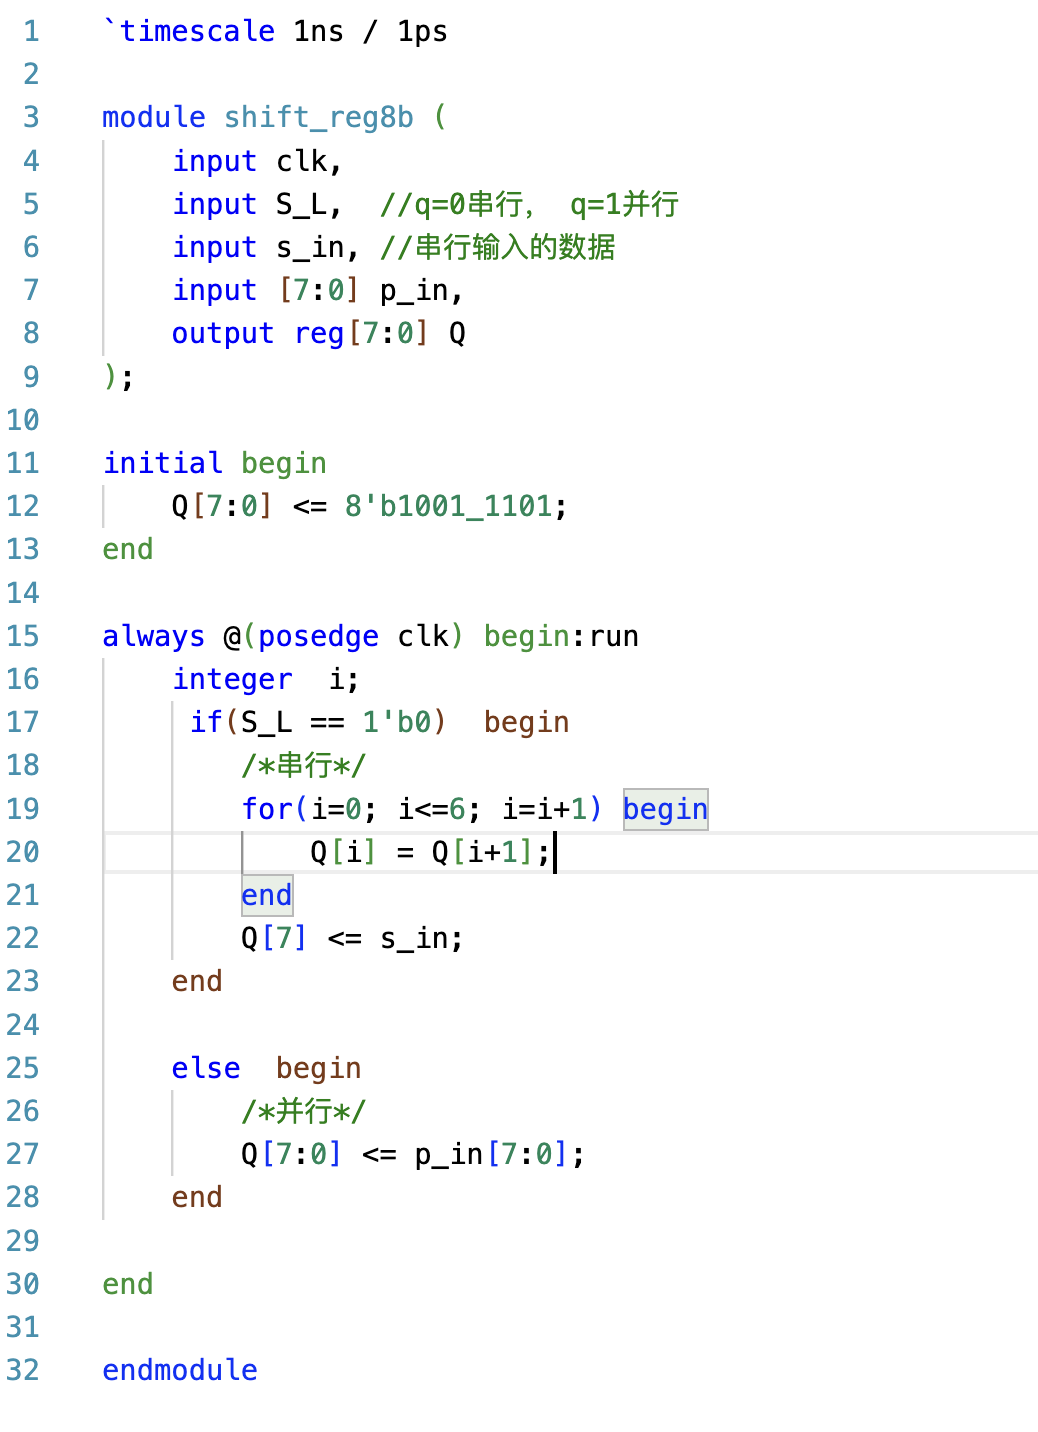
\includegraphics[width=0.4\textwidth]{p1.png}

\end{figure}
当S\_L为0时进行串行输入,s\_in为将要串行输入的数据.

当S\_L为1时进行并行输入,p\_in为并行输入所要输入的数据.

\subsubsection*{sift\_reg8b\_tb.v}
通过testbench得到波形图,对设计的移位寄存器进行分析,测试文件如下:
\begin{figure}[H]
    \centering
    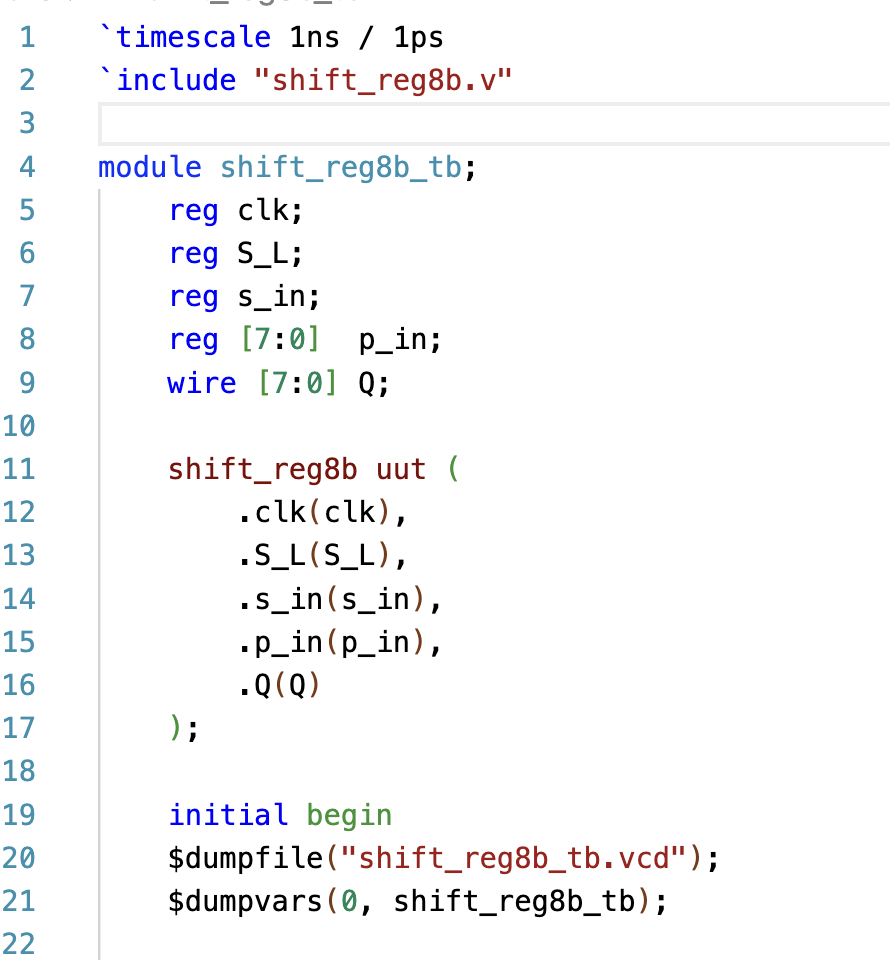
\includegraphics[width=0.4\textwidth]{p2.png}
    
    \end{figure}

    \begin{figure}[H]
        \centering
        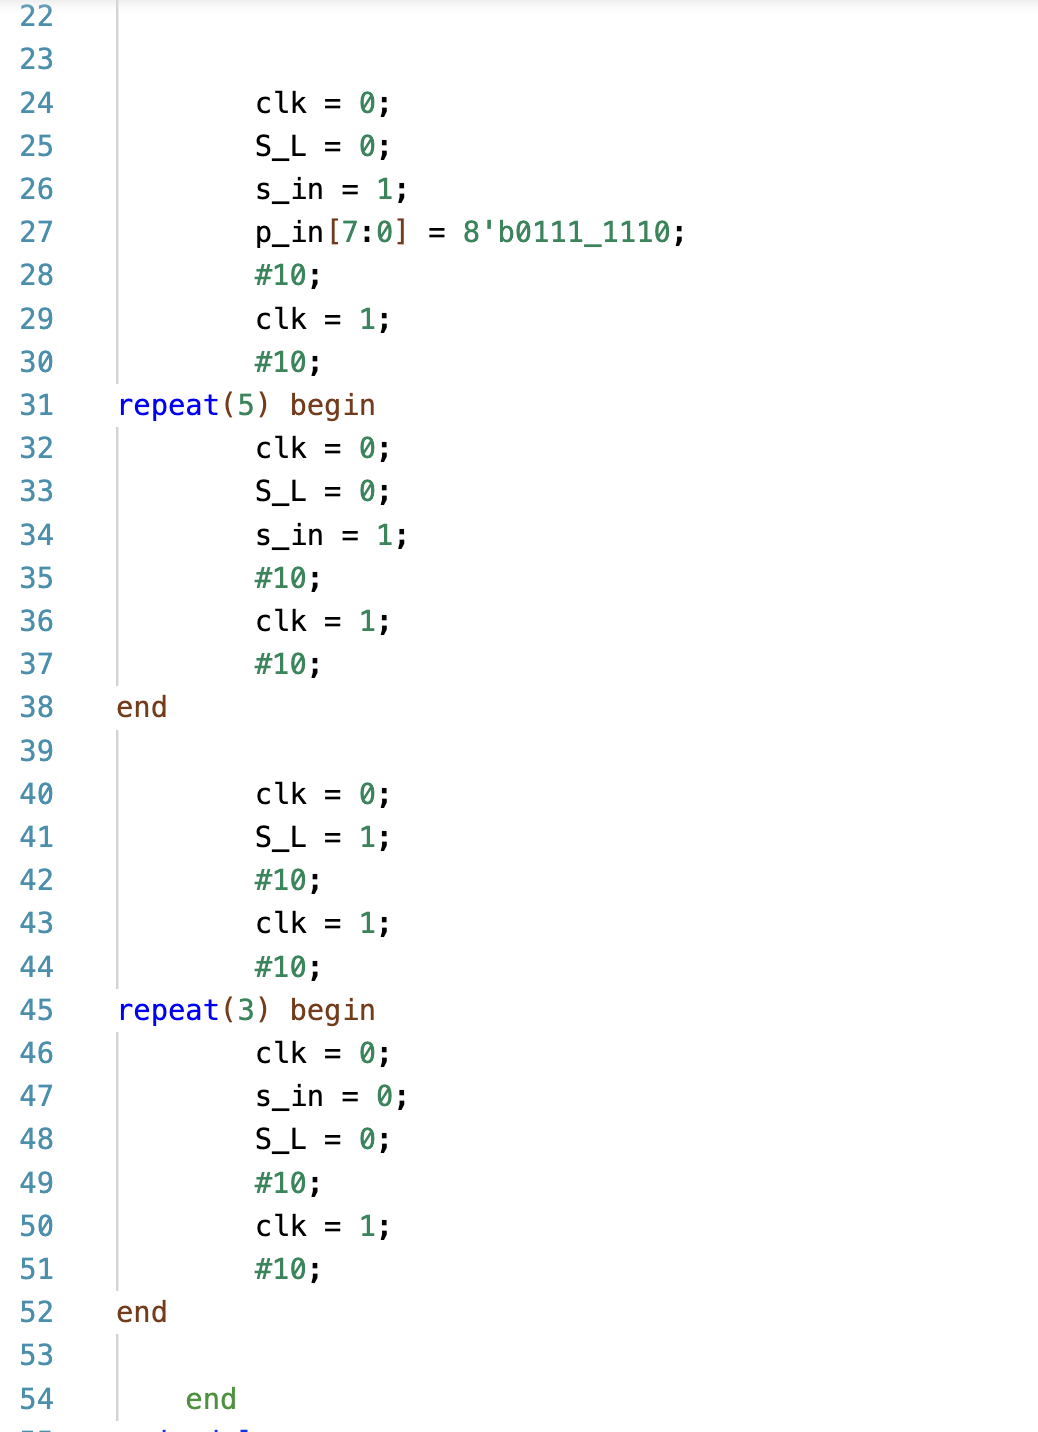
\includegraphics[width=0.4\textwidth]{p3.png}
        
        \end{figure}

\subsection*{任务二:完成P2S模块}

\subsubsection*{完善P2S.v的内容}
将空缺的S\_R锁存器的部分补充完整
\begin{figure}[H]
    \centering
    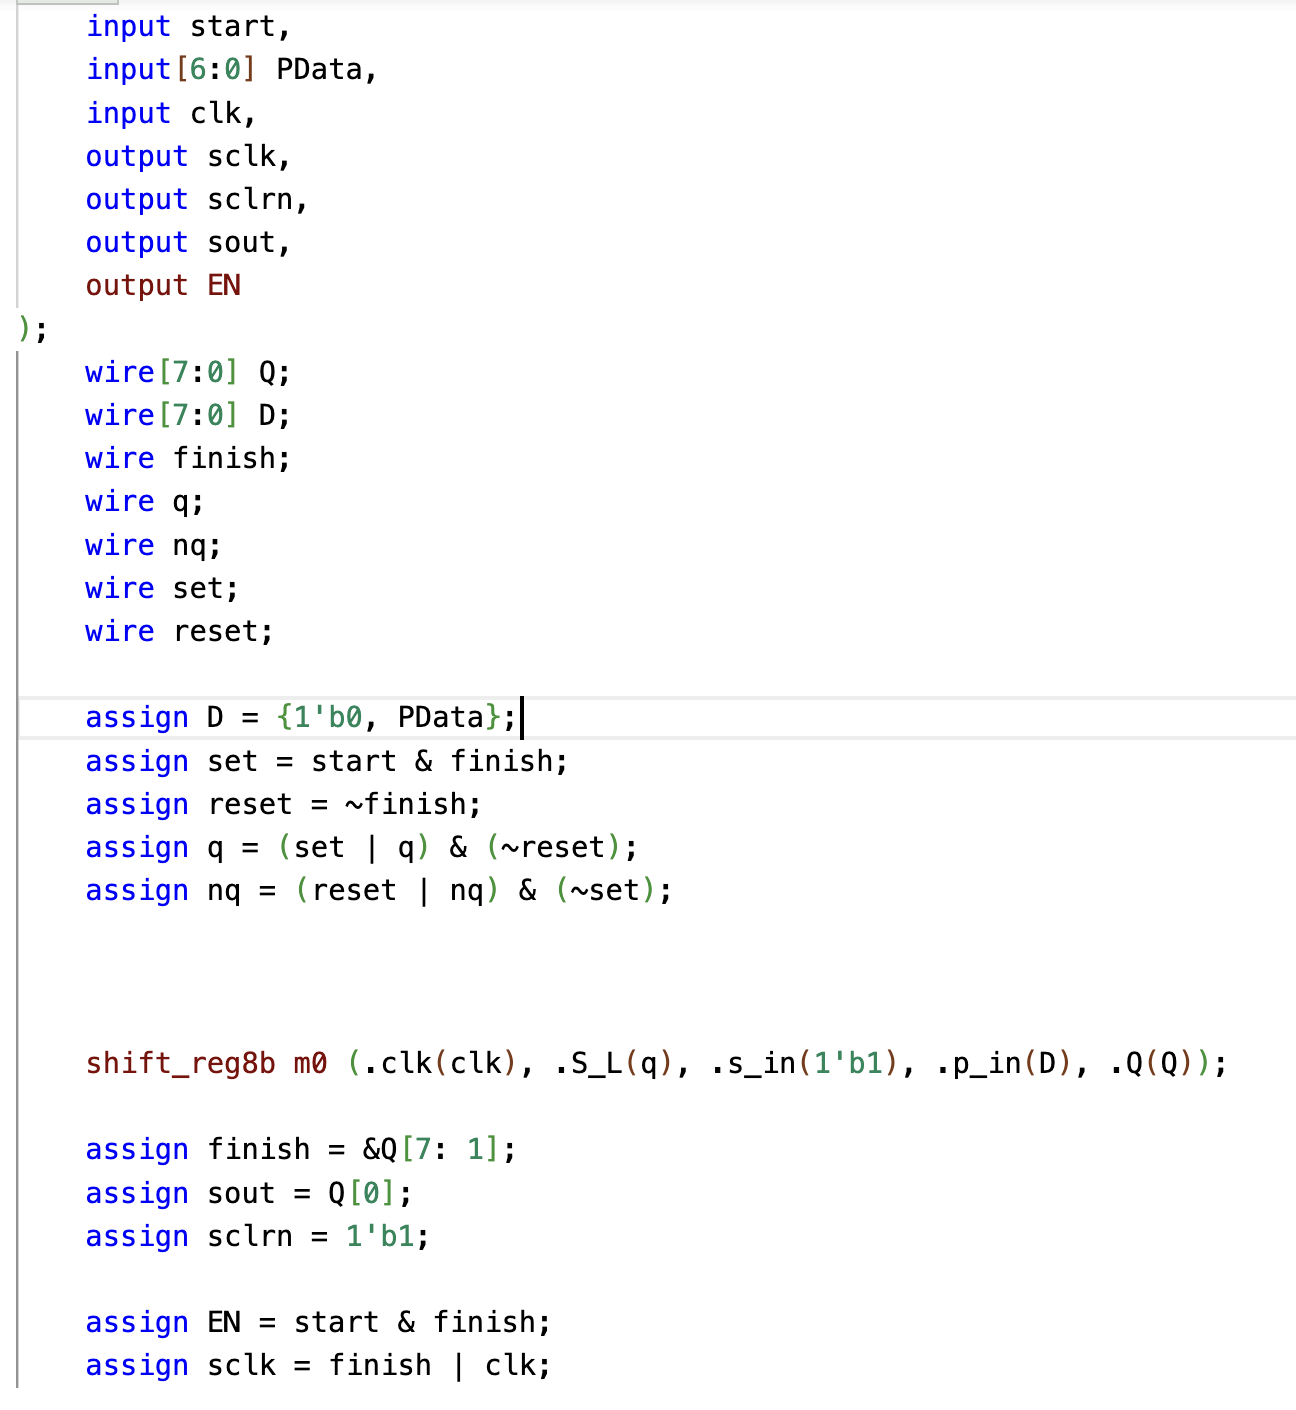
\includegraphics[width=0.4\textwidth]{p4.png}
    
    \end{figure}

\subsection*{d对P2S模块进行测试}
测试代码如下:
\begin{figure}[H]
    \centering
    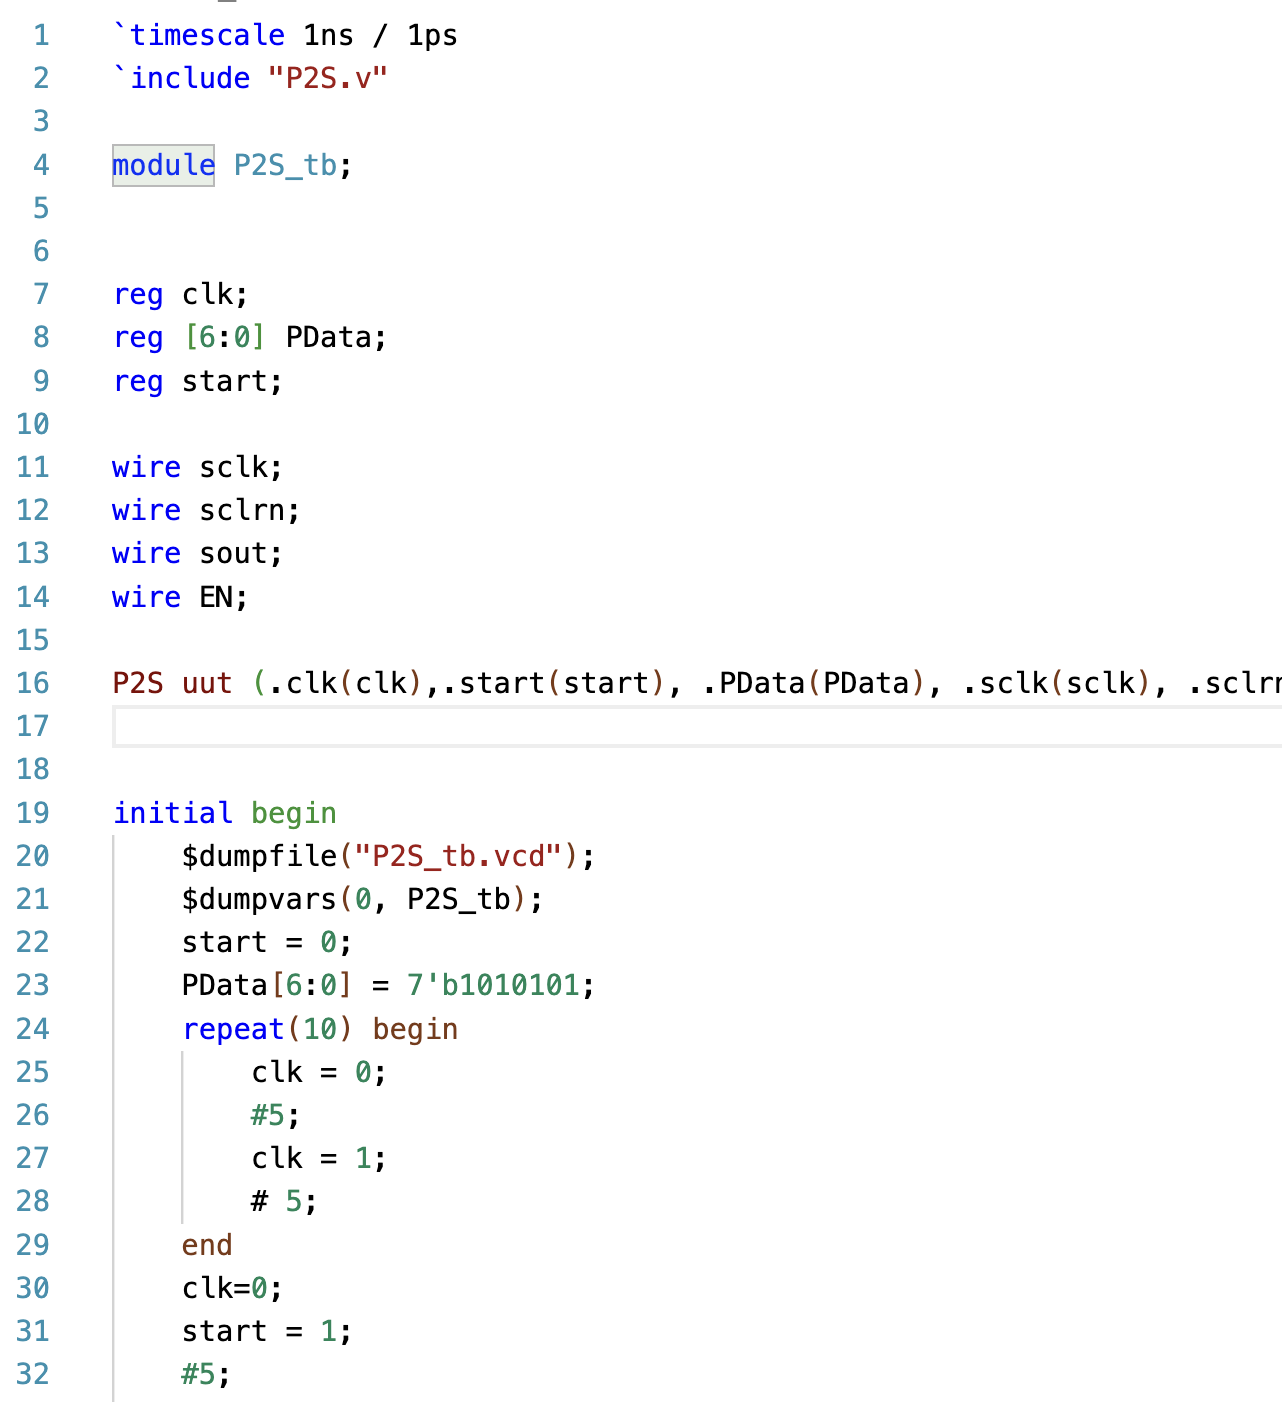
\includegraphics[width=0.4\textwidth]{p5.png}
    
    \end{figure}

 \begin{figure}[H]
        \centering
        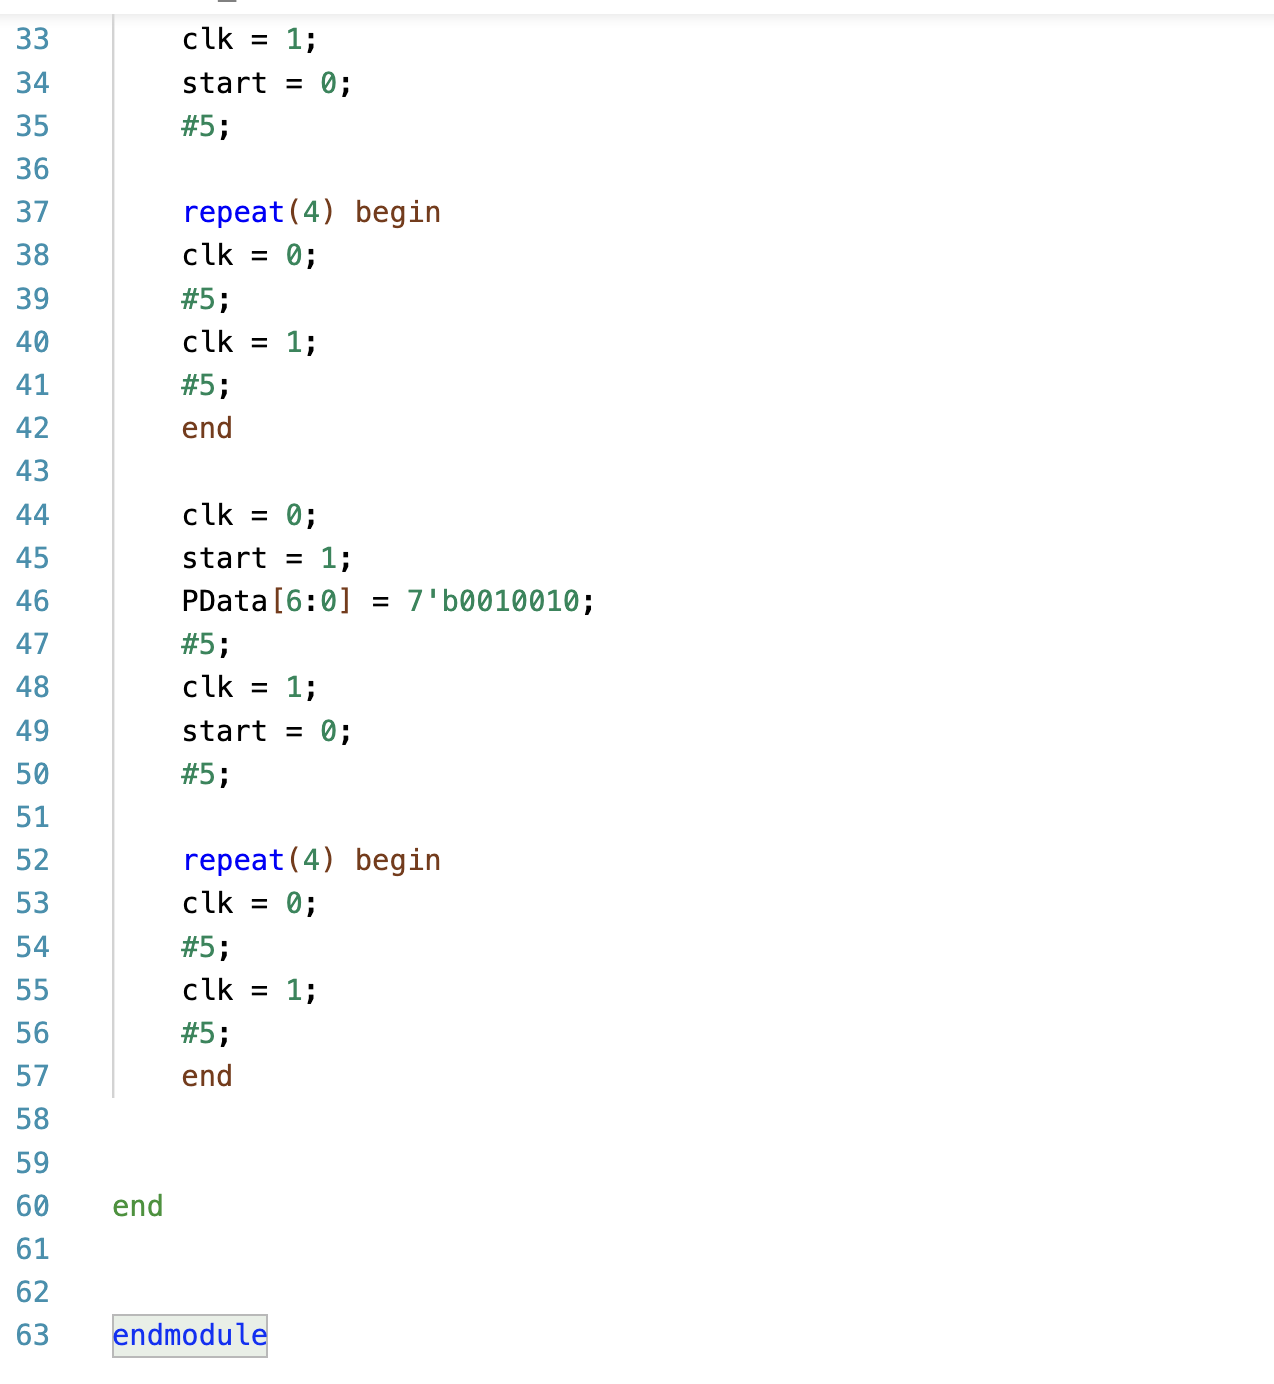
\includegraphics[width=0.4\textwidth]{p6.png}
        
        \end{figure}


\section*{二、实验结果与分析}

\subsubsection*{移位寄存器波形图分析:}
通过测试文件得到波形图,测试的结果如下:
\begin{figure}[H]
    \centering
    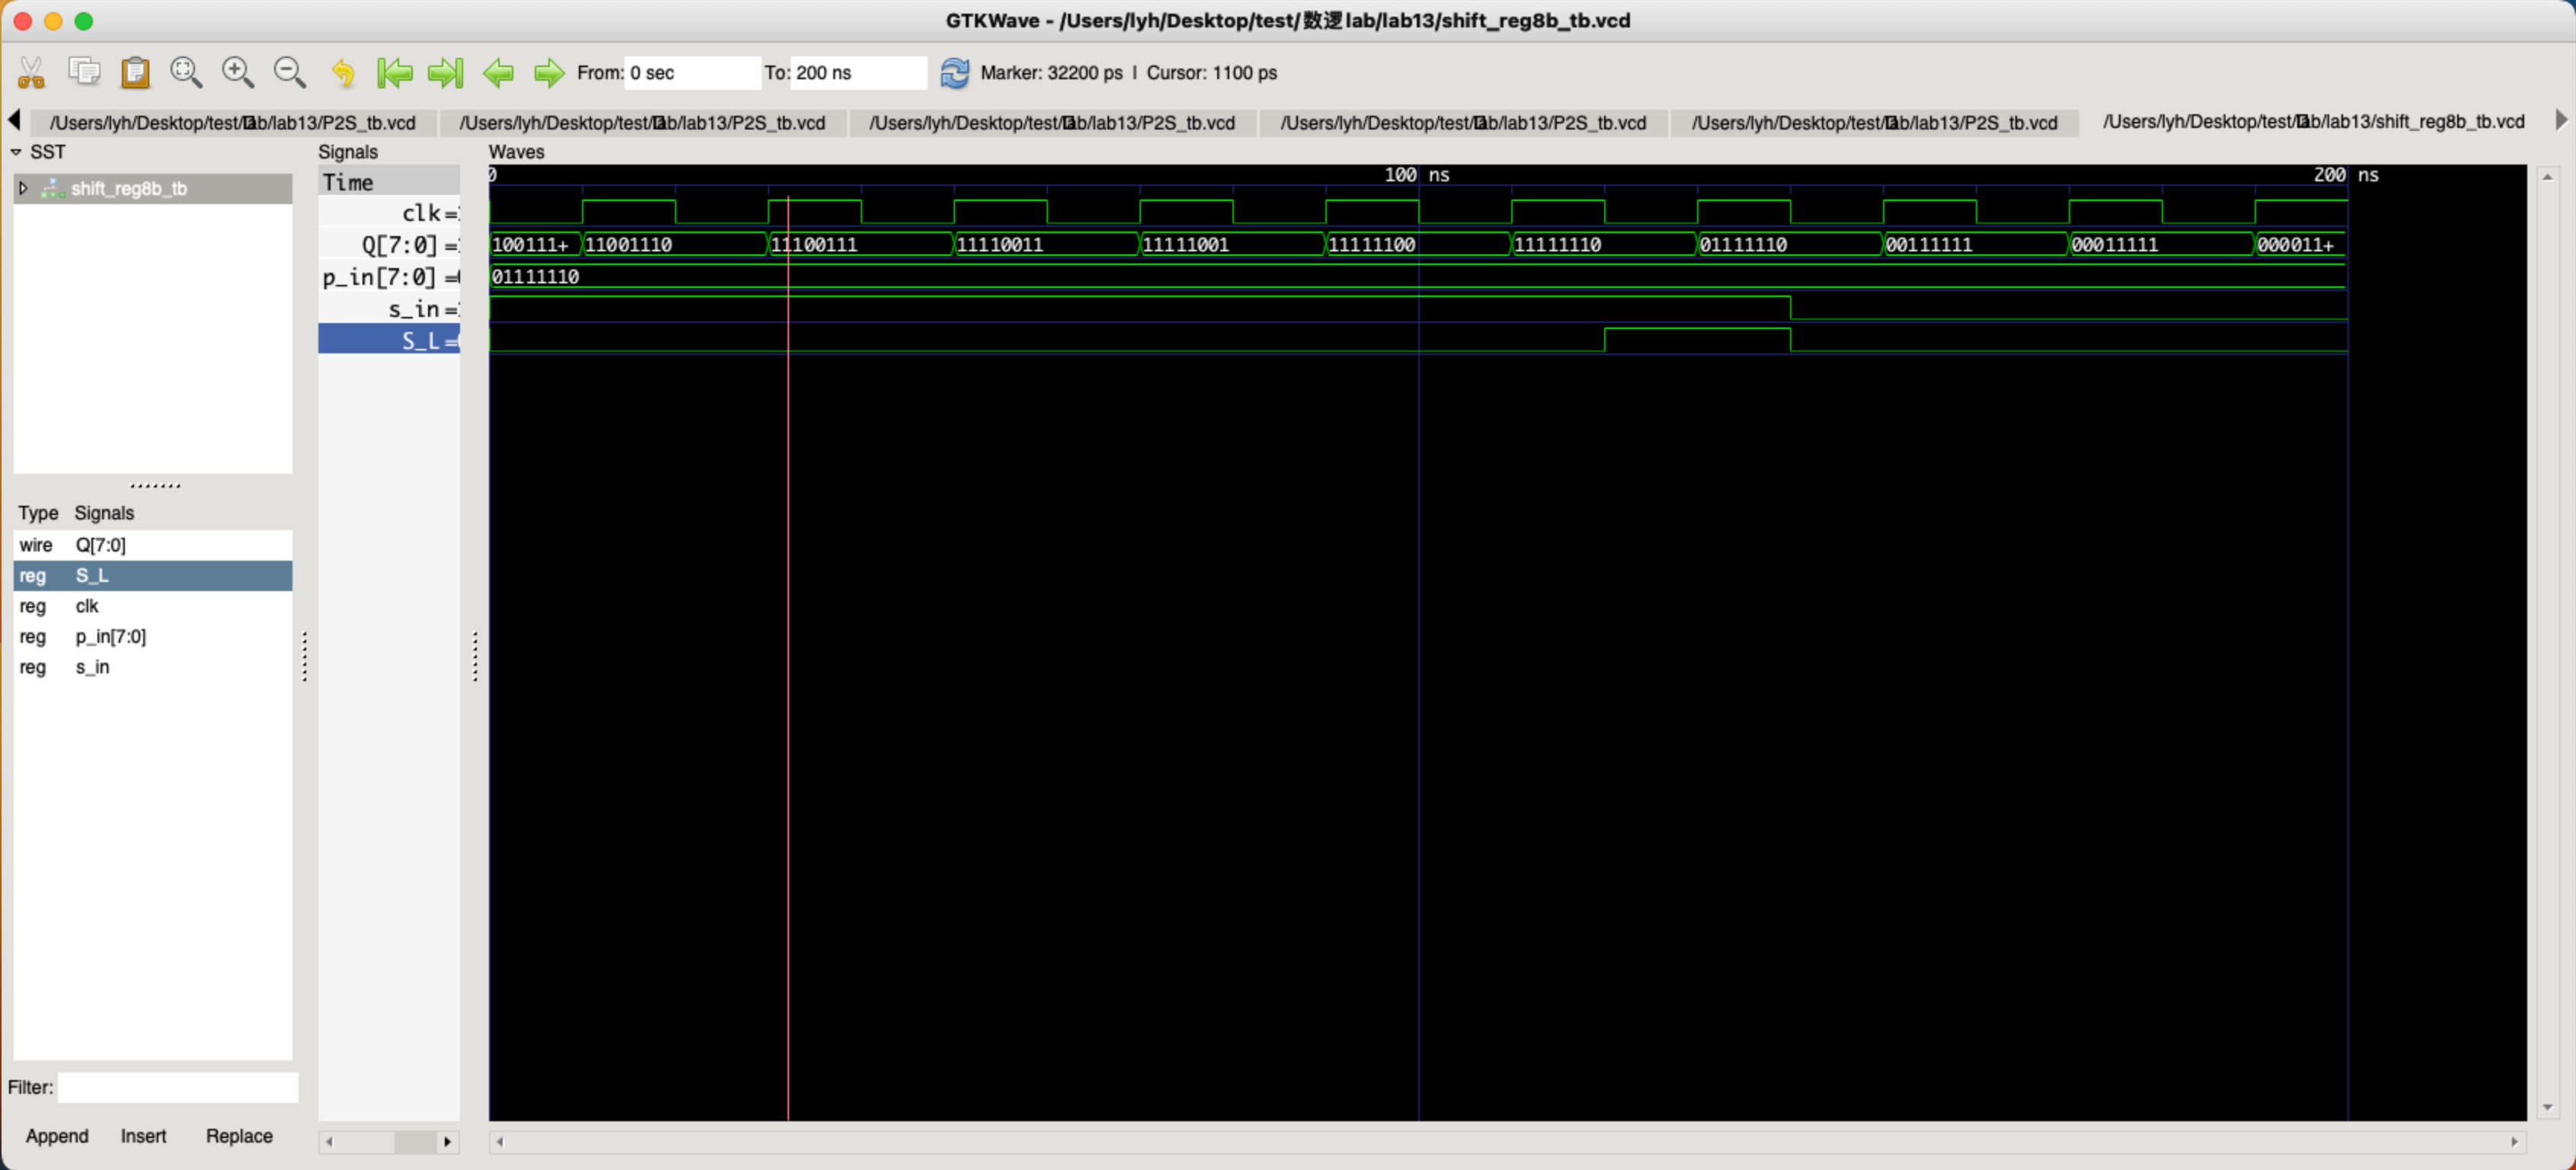
\includegraphics[width=1\textwidth]{t1.png}
    
    \end{figure}
在前六个时钟周期下,S\_L的信号为0,进行串行输入的操作,并且每次串行操作补充的数为1,
输出的结果进行了6次右移,接下来的时钟周期下S\_L的信号为1,进行并行输入的操作,此时p\_in为将要串行输入的数据,
在波形图中可以看出正确进行了传输,接下来后面的时钟周期进行串行输入,并且每次串行输入的数据为0.


\subsection*{P2S模块的波形分析}

\begin{figure}[H]
    \centering
    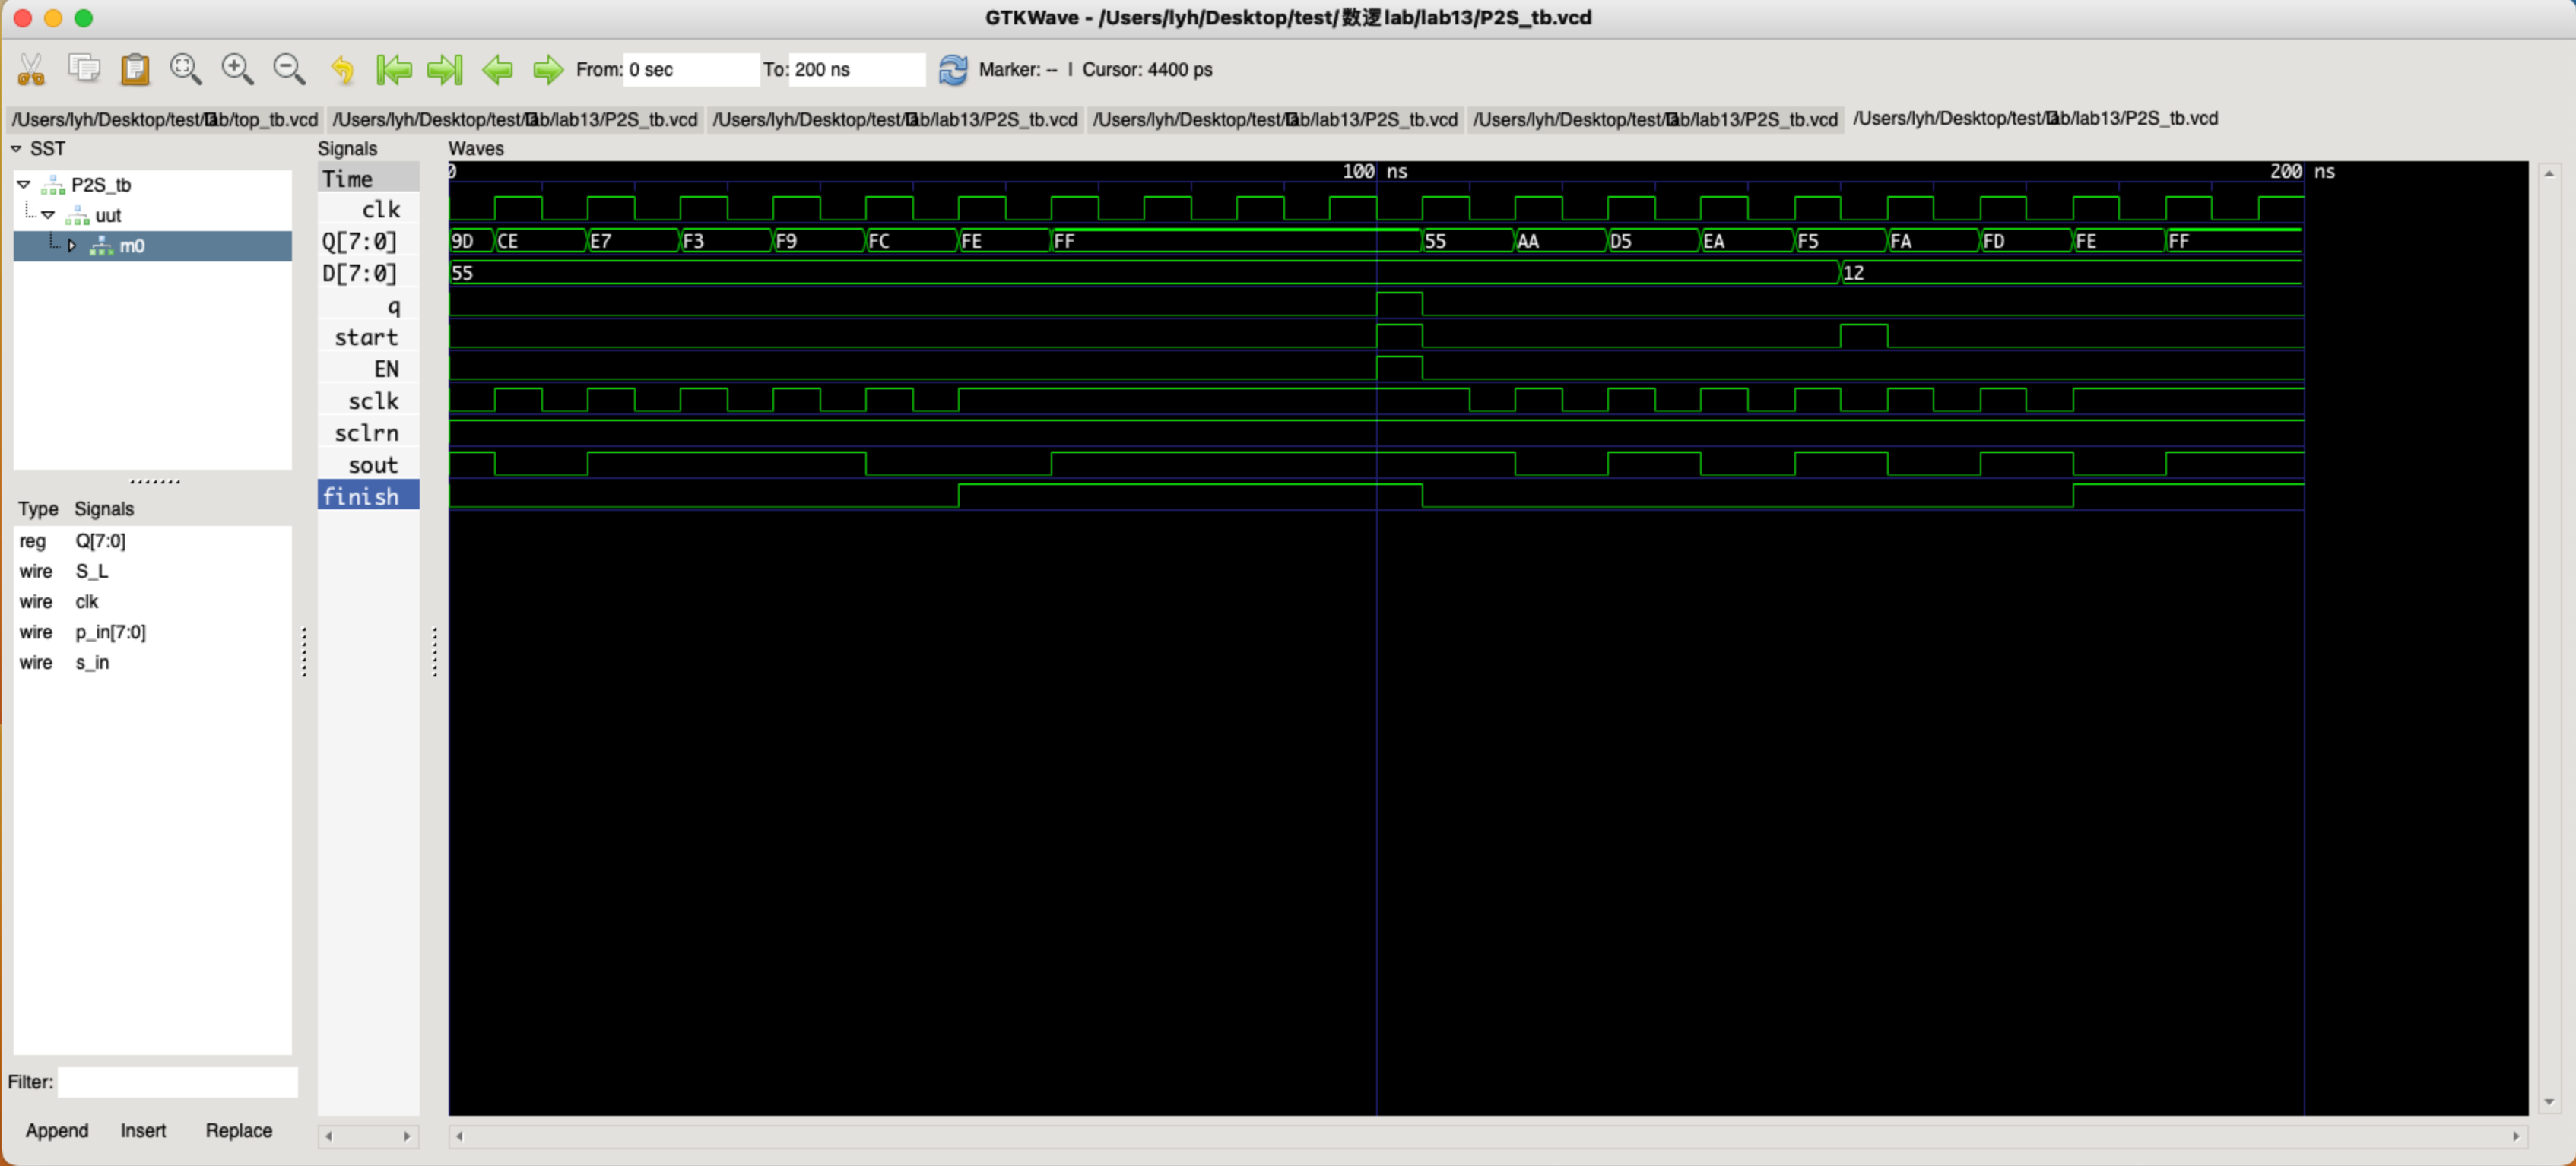
\includegraphics[width=1\textwidth]{t5.png}
    
    \end{figure}


二进制形式的输出结果:
\begin{figure}[H]
    \centering
    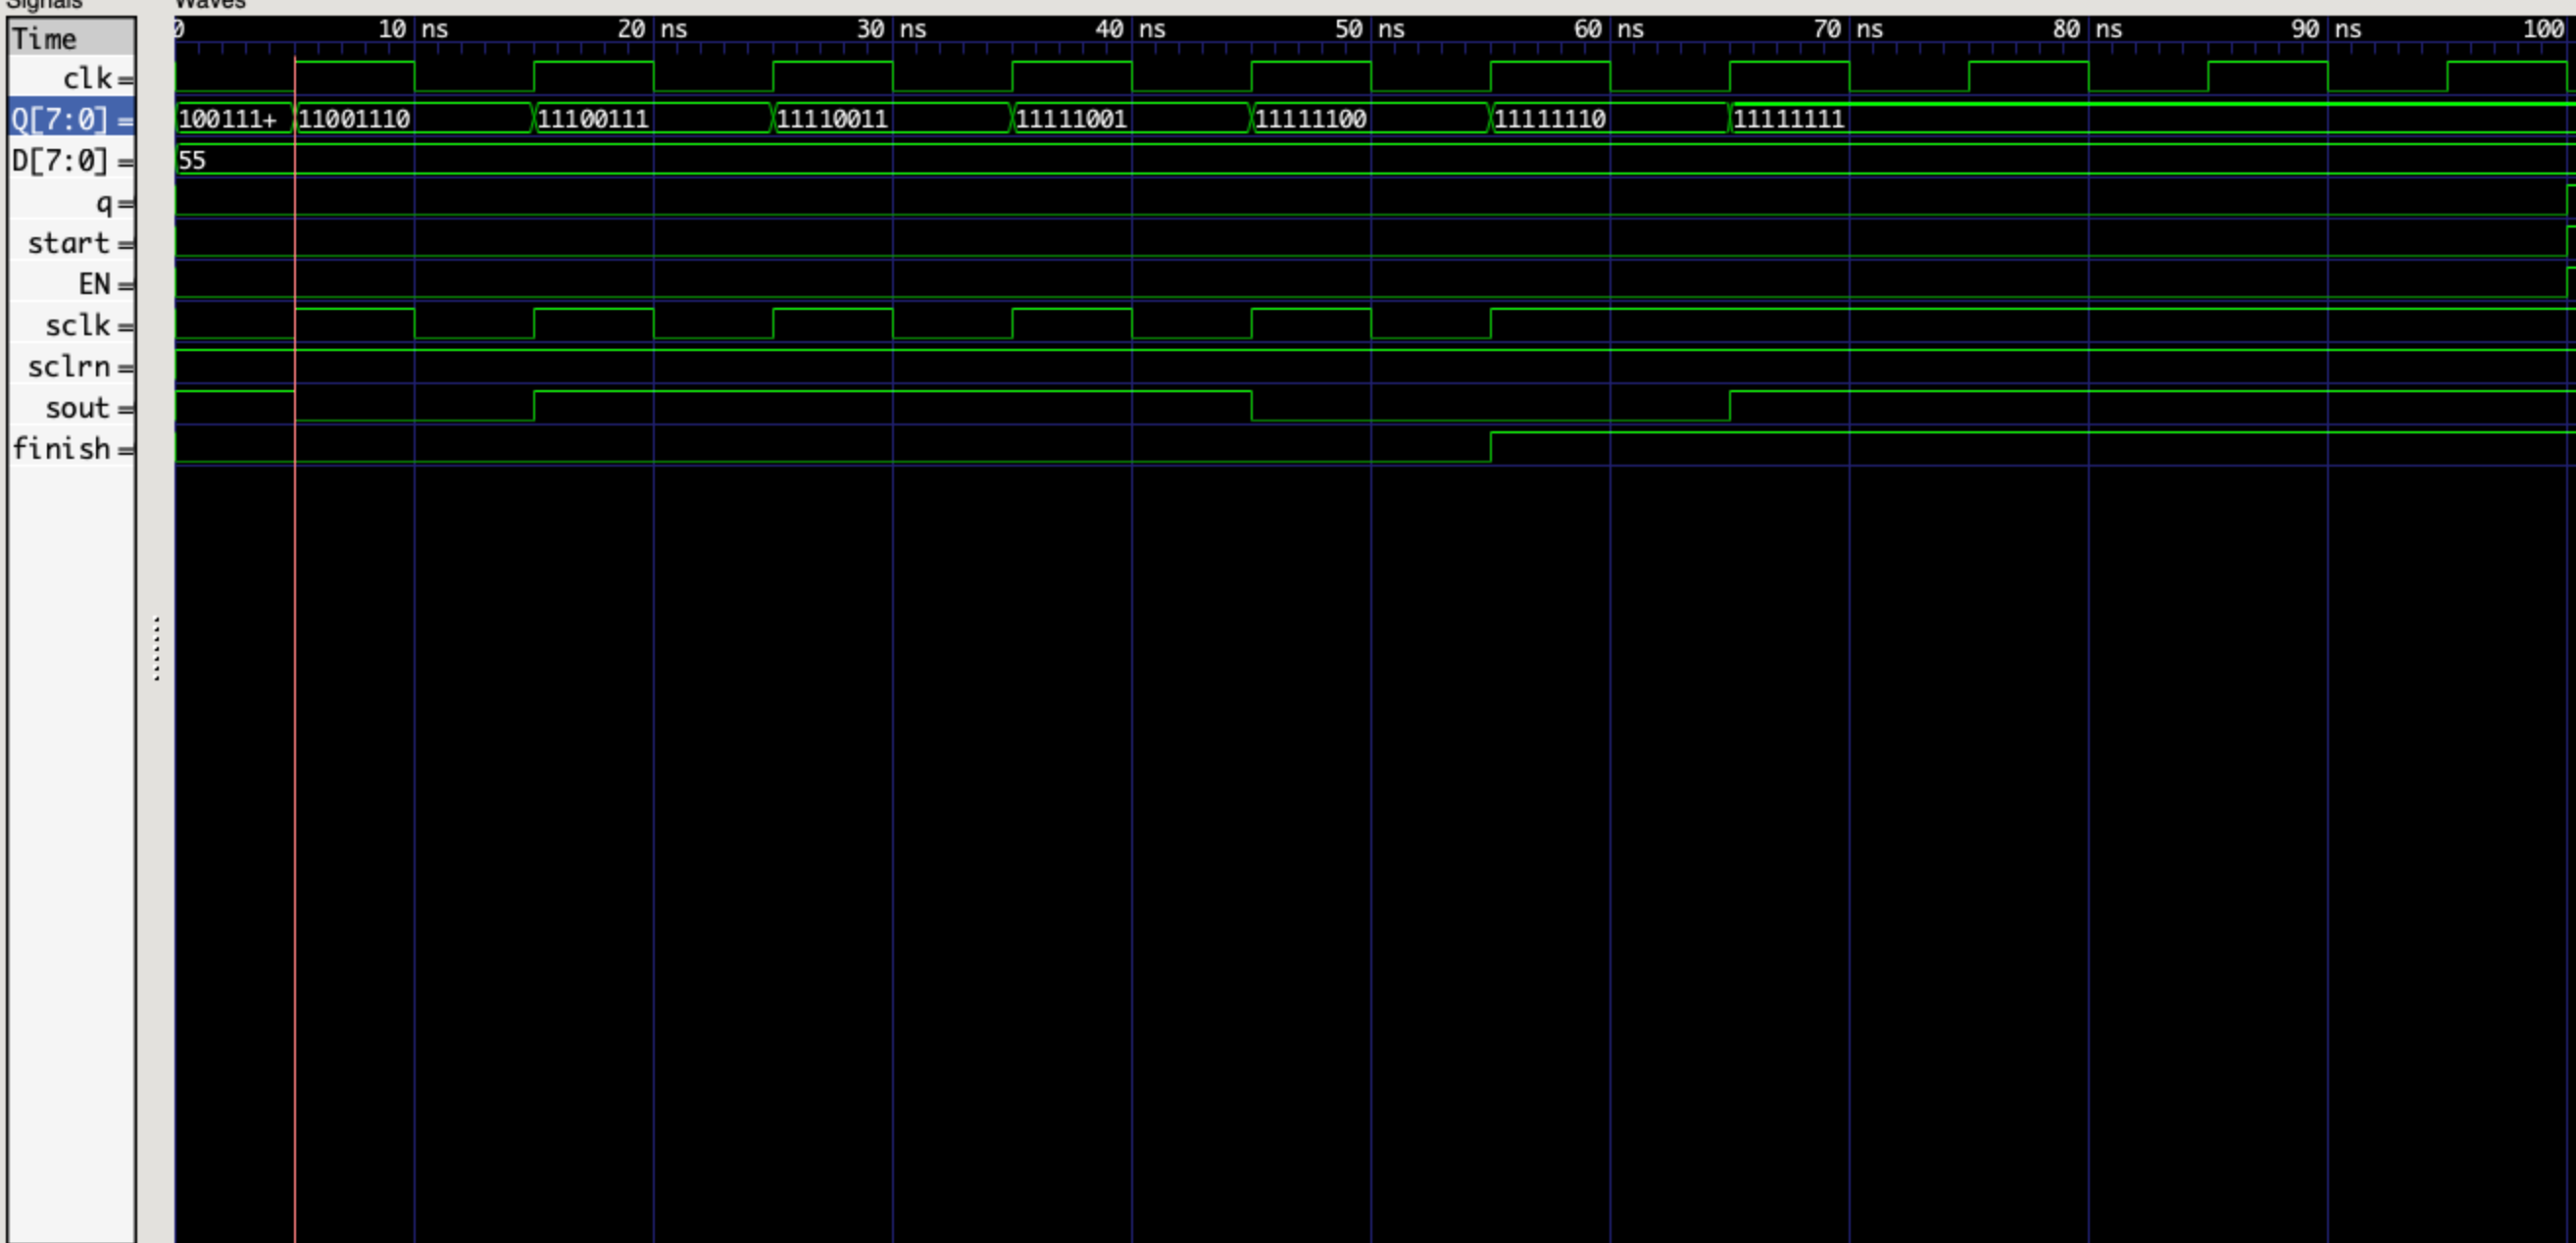
\includegraphics[width=1\textwidth]{t2.png}
    
    \end{figure}

    \begin{figure}[H]
        \centering
        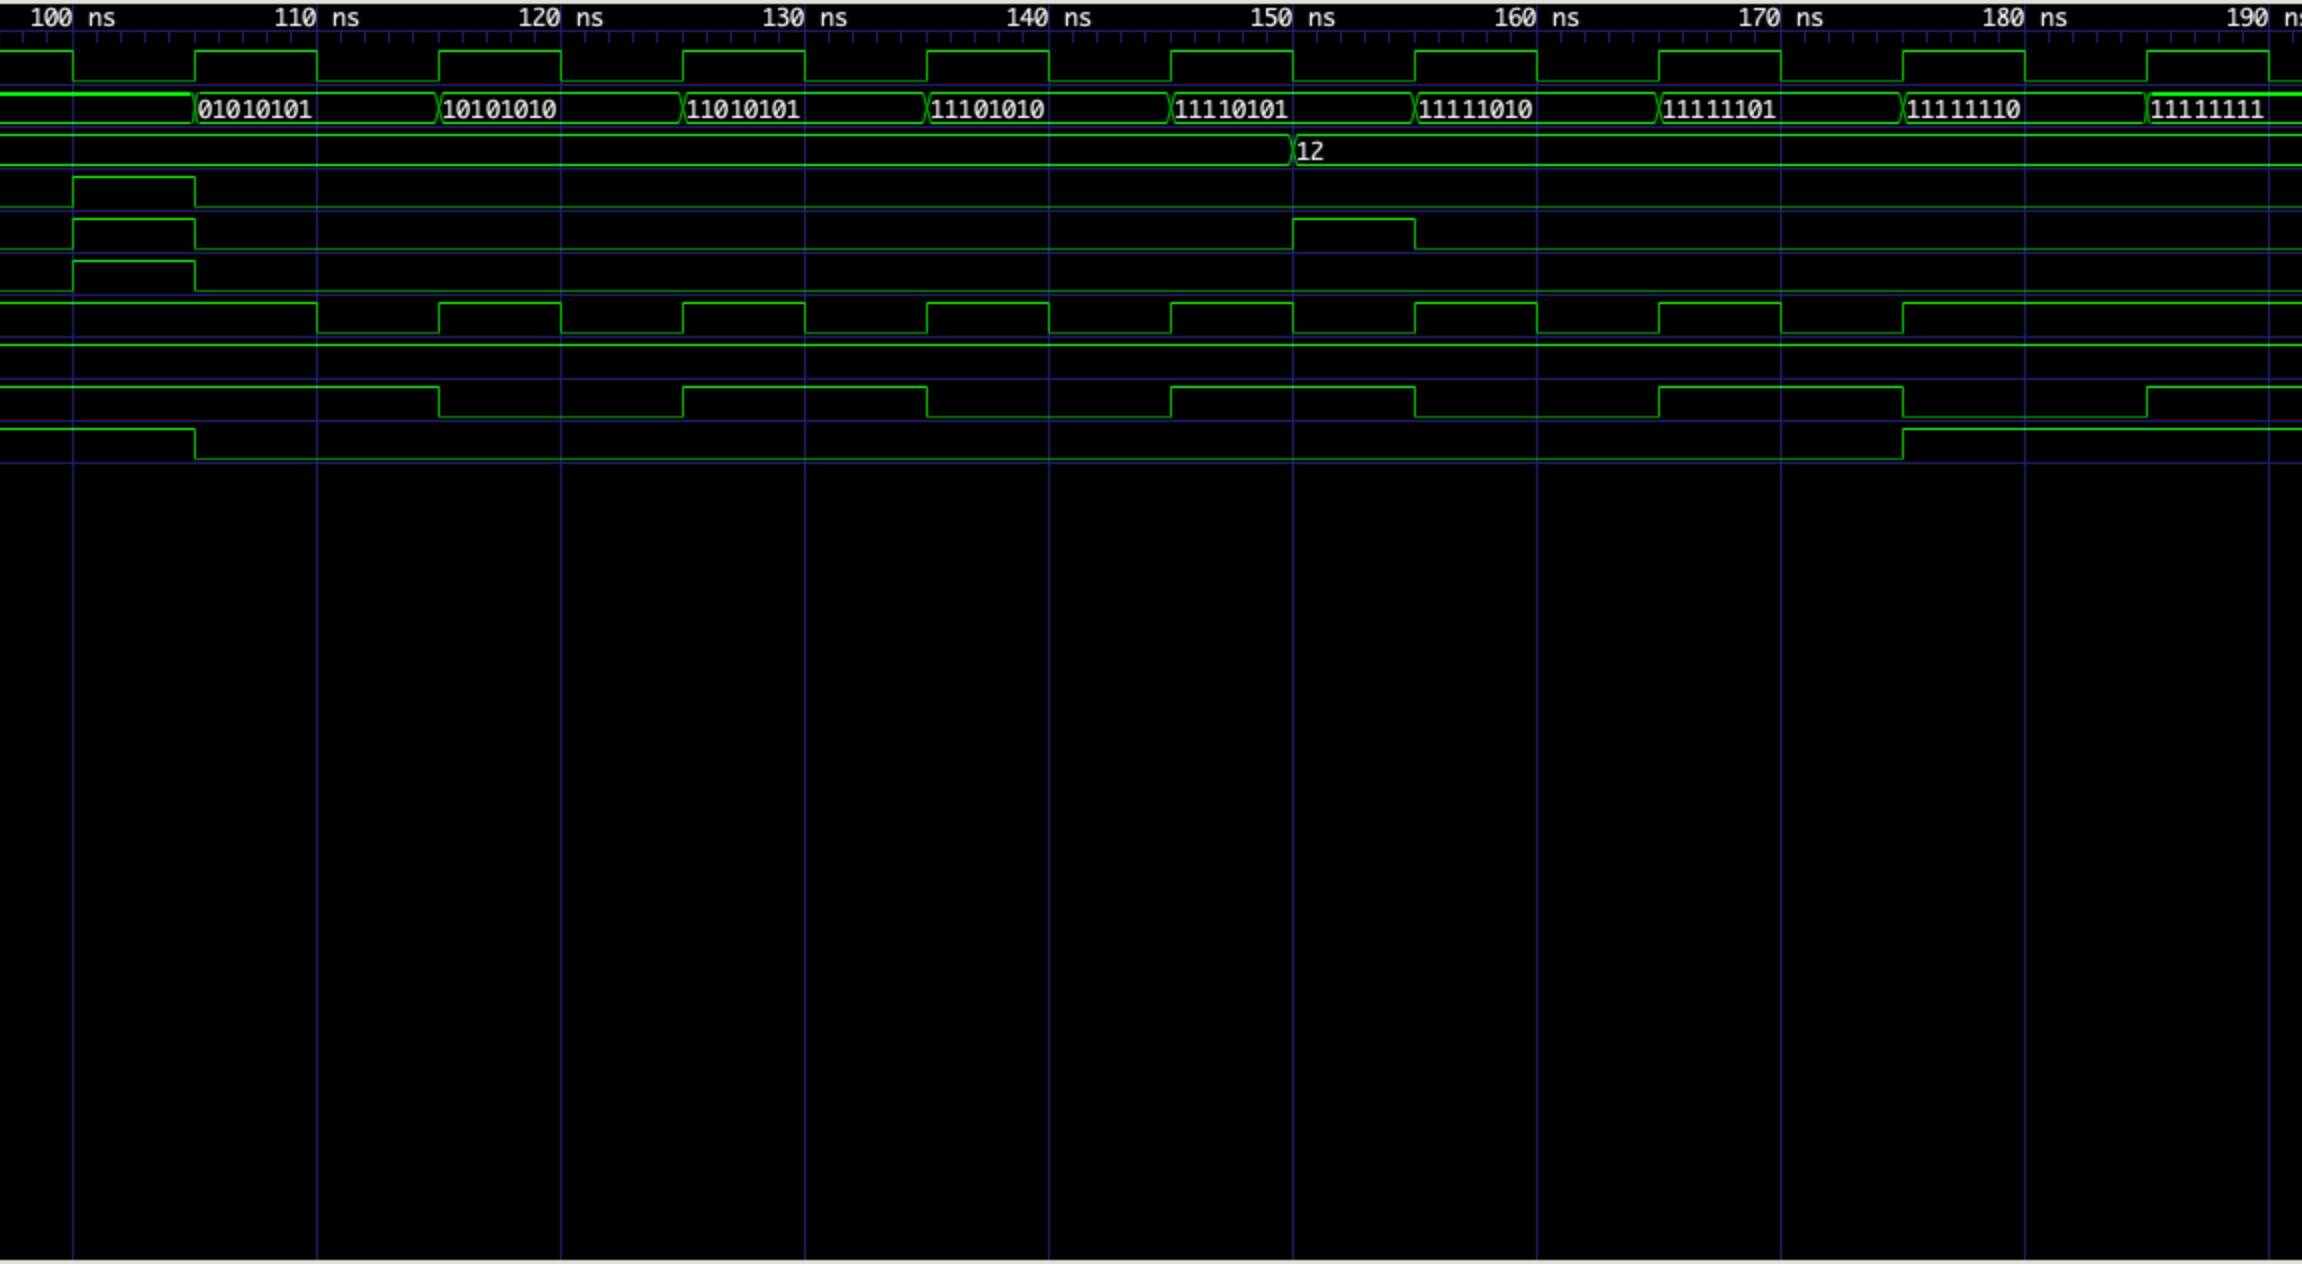
\includegraphics[width=1\textwidth]{t3.png}
        
        \end{figure}

在前7个时钟周期里先进行的串行输入的操作,由于载入数据的信号为0,并且由\&Q[7:1],控制的
finish信号也为0,因此P2S模块中的S\_R锁存器的reset信号为1,set信号为0,因此输出的q信号为0,
进行的是串行输入的模式,并且每次补充的数据都是1,当信号不断移位变成FE时,此时的finish信号为1,
但set信号和reset信号都为0,仍然持续进行移位的操作输出的信号为FF,在其后面的时钟周期里,start信号为1,代表已经准备好了
要输入的数据,并且finish信号也为1,所以set信号为1,p信号此时为1,进行串行载入的模式,可以看到并行的数据被载入到了Q中,在后面的时钟周期中
也出现了一个start为1的状态,但是此时的finish信号为0因此不会进行并行载入的模式,还时持续进行串行输入.

其他输出信号都按照P2S模块中的逻辑进行正常的输出.


\section*{三、讨论与心得}
由于疫情的影响本次实验都通过模拟仿真来进行,实验中完成了移位寄存器和P2S模块,并且进行了模块的仿真,P2S模块的一些内容比较复杂,但在助教讲解之后,
对P2S模块的功能的理解也比较顺利,整体的完整较为轻松.
\end{document}